\chapter{Bend Geometry in Liquid Crystals}
\label{ch:TwistBend}
\section{Introduction}
Geometric structures pervade the physics of liquid crystals. Famously, it was the geometry of focal conics that led Friedel to an understanding of smectics~\citep{friedel1910}. This has been followed by geometric models of developable domains~\citep{kleman80,bouligand80}, screw dislocations and grain boundaries~\citep{kamien99}, columnar phases on curved substrates~\citep{santangelo07}, and the beautiful explanation of the frustration in blue phases \citep{sethna83}. The geometry of vector or nematic-like order was introduced in \S\ref{subsec:Geometry} where we gave Frank's elasticity of nematics \eqref{eq:FrankFreeEnergy}, in which the fundamental modes of distortion --- splay, twist, bend, biaxial splay --- are named for their geometric character. Corresponding to the symmetries of this elasticity we had the decomposition \eqref{eq:GradientDecompositionpar}, \eqref{eq:GradientDecompositionperp} of director gradients into components parallel ($\nabla^L \w n$) and perpendicular ($\nabla^\xi \w n$) to $\w n$. Focusing on the shape operator $\nabla^\xi \w n$, we saw that there were geometric singularities called umbilic lines \citep{Machon2016b}, zeros of the deviatoric part of $\nabla^\xi \w n$, $\Delta$, which describes directions of principal curvature. The importance of umbilic lines is brought to the fore when they have direct energetic consequences, as in a cholesteric liquid crystal, minimally described by 
\begin{equation}
    F_{\mathrm{ch}} = \frac{K}{2}  \int d^3 {\bf r}\left(|\nabla {\bf n}|^2 +2 q_0 {\bf n} \cdot \nabla \times {\bf n} \right),
    \label{eq:CholestericFreeEnergy}
\end{equation}
a modification of \eqref{eq:FrankFreeEnergy} in which all elastic constants are set to the same value $K$ and the twist energy is shifted to have a minimum at $\w n \cdot \nabla \times \w n = -q_0$ \citep{deGennes1992}. The groundstate is given by any director field equivalent to $\w n = (\cos q_0 z, \sin q_0 z, 0)$ (with nonzero twist $q_0$), where the local $z$ direction is set by the pitch axis, $\w p$, a second vector distinct from the line field $\w n$ which gives the local axis of twisting in the cholesteric. The eigenvectors of $\Delta$ determine $\w p$ \citep{Bellar2014, Machon2016b}, and umbilics in cholesterics then correspond to energetically costly defects in the pitch axis called $\lambda$ lines \citep{Bellar2014}. Cholesterics themselves support an increased variety of metastable states relative to the nematic phase, with many topological configurations including Skyrmions, Hopfions and other knotted solitons (some of which are shown and discussed in \S \ref{subsec:SkyrmionsAndHopfions}), novel textures of shells and droplets, and constellations of point defects~\citep{posnjak17}. Within these solitons, $\lambda$ lines might be considered `fingerprints', naturally localised geometric structures describing energetic frustration, which also convey global topological information about the texture as zeros of a section of the nontrivial part of $\xi^* \otimes \xi$ directly derived from $\w n$. 

This chapter is about the geometry and topology in the part of $\nabla \w n$ not examined above, $\nabla^L \w n= \w n^* \otimes \nabla_\w n \w n$, determined by the bend vector $\w b:= \nabla_\w n \w n$. By analogy with the description of the shape operator, umbilic lines and cholesterics given above, several questions suggest themselves: If the geometry of $\Delta$ is the geometry of surface curvatures, what is the geometry of $\w b$? Do cousins of umbilic lines exist, and if so what is their structure and topological significance? What types of `bend solitons' might we expect? And, if cholesterics are the natural setting to study umbilics, what is the natural setting to study bend? The recently discovered twist-bend nematic~\citep{Cestari2011, Chen2013, Borshch2013, Lavrentovich2018} is one answer to this last question, providing a system in which the geometry of bend is naturally brought to prominence. In these systems the molecules have a bent-core architecture that leads to an energetic preference for non-zero bend. The observed phase, and apparent theoretical groundstate, has a heliconical ordering that is intermediate between ordinary nematics and cholesterics. As such, we might expect analogous textures and topological states to those observed in cholesterics. One key difference between the systems, however, is that the cholesteric energy \eqref{eq:CholestericFreeEnergy} is intrinsically chiral --- left handed and right handed twist have different energies. By contrast, the twist-bend nematic energy is achiral, the ground state spontaneously picking one of two equal energy heliconic (hence chiral) states. A second difference is that the bend is identically zero in the cholesteric ground state.

In \S\ref{sec:Elements} we will describe the fundamental geometry and topology of bend, relating it to the curvatures and torsions of families of integral curves, and show that cousins of umbilic (or $\lambda$) lines exist, which we call $\beta$ lines. Their structure, including a natural notion of self-linking, will be discussed in \S\ref{sec:TheStructureOfBendZeros}. These $\beta$ lines, zeros of a section of $\xi$, provide topological information analogous to umbilics; they give a Skyrmion count, and are capable of distinguishing textures of different Hopf invariant. We explore their topological significance in \ref{sec:TopologicalSignificance}. Throughout, we will use the twist-bend nematic as a model system, providing simulation results of twist-bend Skyrmions and Hopfions. As such, we give a standalone introduction to twist-bend nematics in \S\ref{sec:TwistBendNematics}. 

\section{Elements of the global geometry and topology of bend} 
\label{sec:Elements} 
We firstly specify a few technical details brushed over in \S \ref{subsec:Geometry}. Vector bundles over a contractible space (like $\mathbb{R}^3$) are trivial \citep{MilnorStasheffBook}, as are homotopy classes of maps from this space into any other (in our case specifically $S^2$ or $\mathbb{R}P^2$)~\citep{Hatcher2012}. So in order to see topologically interesting features, such as a nontrivial Euler class for $\xi$, our material must be topologically nontrivial. We will denote it by a general 3-manifold $M$, and typically have in mind experimentally accessible examples like $S^3, D^2 \times S^1$, $S^2 \times S^1$, perhaps also $T^2 \times S^1$ or $T^3$, as well as the plethora of 3-manifolds given by knot complements\footnote{Not all of these examples actually can support nontrivial $\xi$! For example, $H^2(S^3)=0$.}. $M$ has a metric, which we denote $\langle \bullet , \bullet \rangle$ or, when using vectors and there is no chance of ambiguity, with the dot product notation $\bullet \cdot \bullet$. The manifold is considered equipped with its standard metric compatible connection $\nabla$. We will also freely use vectorial and vector calculus notions such as cross products, gradients and curls, for example writing $(\w n \cdot \nabla \w) \w n = \nabla_{\w n} \w n$, where on the left hand side with have the vector calculus gradient and dot product, and on the right the connection. These vectorial concepts may be defined on a general 3-manifold in terms of differential forms, wedge products and so forth \citep{Lee1996, Frankel2015}, however typically we think of our 3-manifold as a subset of $\mathbb{R}^3$ with some nontrivial boundary conditions which allow us to compactify the space (for example imposing fixed far field boundary conditions on $\mathbb{R}^3$ allows compactification to $S^3$). As such, we may locally consider the manifold $\mathbb{R}^3$ with its standard connection and metric, and think of vectorial notions in the familiar direct way, moving freely between them and the alternative presentation involving connections and differential forms. 

\label{sec:TheStructureOfBendZeros}
The bend is the change of the director field along itself, ${\bf b} = \nabla_{{\bf n}}{\bf n}=-{\bf n}\times\nabla\times{\bf n}$, and is a globally defined vector whose sign does not reverse under the replacement of ${\bf n}$ by $-{\bf n}$. As such, it is well defined for a line field, however in this chapter we will restrict our attention to orientable textures (those without disclination lines) in which $\w n$ can be considered a unit vector. As ${\bf n}$ is a unit vector, the bend is everywhere orthogonal to it, ${\bf b}\cdot{\bf n}=0$ --- that is, $\w b$ is a section of $\xi$. Setting ${\bf b}_\perp:={\bf n}\times{\w b}$ and denoting their normalised vectors ${\bf e}_1 := \w b/|\w b|$, $\w e_2 := \w b_\perp/|\w b_\perp| = \w n \times \w e_1$ we have a local orthonormal frame $({\bf e}_1, {\bf e}_2, {\bf n})$. Considering a single integral curve of the director, this frame is exactly the Frenet-Serret frame $({\bf e}_1, {\bf e}_2,{\bf n}) = (\w N, \w B, \w T)$ \citep{DoCarmoBook}, where $\w T, \w N, \w B$ are the tangent, normal and binormal to the integral curve, and in terms of curve geometry $\w b = \kappa \w N$, where $\kappa$ is the classical curvature. Continuing in the same vein, the torsion of the integral curves is given by $\tau  = \langle \w e_2 , \nabla_\w n \w e_1 \rangle $, a measure of how the Frenet-Serret frame spins about the tangent as one moves along the curve. For any curve, its torsion $\tau$ may be interpreted as the connection one form corresponding to the restriction of the ambient connection onto the curve's normal bundle. For the family of integral curves given by the director we interpret it as one component of a connection one-form on the bundle $\xi$,  
\begin{equation}
    A := \langle \nabla \w e_1 ,\w e_2 \rangle = \frac{\langle \nabla \w b ,\w b_\perp \rangle}{\langle \w b,\w b \rangle}. 
    \label{eq:1form}
\end{equation}
This 1-form and its associated curvature $\Omega = dA$ will enter in a fundamental way into the characterisation of the director field, orienting bend zeros and giving a count of Skyrmions. A few remarks about \eqref{eq:1form} are in order. Firstly, the connection $\nabla$ here is a connection on the bundle $\xi$, and is globally well defined as the restriction of the ambient connection on the manifold to the plane field $\xi$. Equivalently, it is the pullback connection induced by the map ${\bf n}: M \rightarrow S^2$ \cite{Lee1996}.\footnote{$\w n$ is a unit magnitude section of $TM$. However, 3-manifolds are parallelisable \citep{Geiges2009}, meaning an everywhere nonzero basis can be chosen for the entire bundle. Relative to such a basis $\w n: M \rightarrow S^2$.}. The sections $(\w e_1,\w e_2)$ are, however, only well defined on the complement of the bend zeros (which we come to in a moment), and this carries through to the 1-form $A$. 

The bend is a vector in three-dimensional space, and a generic such vector vanishes at isolated points. However, the constraint that it be orthogonal to the director makes it atypical, having only two degrees of freedom --- $\w b$ is locally a map $\mathbb{R}^3 \rightarrow \mathbb{R}^2$. As a result, the set of points where it vanishes is one-dimensional and forms a set of fundamental curves in the material that are characteristic of the director field. On these lines $\w b = \kappa \w N = 0$, so they correspond to points of inflection in the integral curves of ${\bf n}$, where the curvature $\kappa$ vanishes. We might think of these zeros as `inflectional lines', but we shall refer to them as $\beta$ lines by informal analogy with $\lambda$ lines. Finally, as discussed in \S\ref{subsec:Geometry}, the zeros of any section of an (orientable) vector bundle encode its Euler class. More precisely, the $\beta$ lines, counted with appropriate sign, are Poincar\'e dual to the Euler class of $\xi$, $e(\xi) \in H^2(M)$ \cite{BottTuBook,Hatcher2012, Geiges2009}. This is certainly true, however the $\beta$ lines are more than this --- they are not just any section, freely chosen within $\xi$. Rather, they are directly derived from the director $\w n$, and cannot be varied independently of it. One thus expects them to encode more information than an arbitrary section of $\xi$; we shall return to this point in \S\ref{sec:TopologicalSignificance}. 
\section{Twist-bend nematics} 
\label{sec:TwistBendNematics}
The twist-bend nematic, $N_{\mathrm{tb}}$, is a recently discovered phase of liquid crystal in which the director adopts a spontaneous nonzero magnitude of bend \citep{Lavrentovich2018}. Originally suggested by Meyer \citep{Meyer1976}, the idea was not actively pursued until an article of Dozov's \citep{Dozov2001} in which he considered the possibility of the bend elastic constant, $K_3$ in \eqref{eq:FrankFreeEnergy}, becoming negative, with the free energy then stabilised from below by higher order derivatives. Everywhere constant magnitude bend is not possible in two dimensions \citep{Niv2018}, however provided one accepts an accompanying twist or splay deformation, it is possible in three dimensions. Of these possibilities Dozov focused on the twist-bend case, predicting a heliconical director shown in figure \ref{fig:Bananas}(a)
\begin{equation}
\w n = (\sin \theta \cos q z, \sin \theta \sin q z , \cos \theta),
\label{eq:TwistBendDirector}
\end{equation}
where $2\pi/q$ is the heliconical pitch and $\theta$ is the tilt angle. The bend vector in this heliconical state is $\w b = q\sin \theta \cos\theta (-\sin q z, \cos q z, 0)$ and the twist is $- q \sin^2 \theta$. As $\theta \rightarrow 0$ we recover a simple nematic, and as $\theta \rightarrow \pi/2$ we obtain the cholesteric ground state. A more recent theoretical approach, closer in spirit to Meyer's original work, is to keep $K_3$ positive but augment the director $\w n$ with a vector order parameter $\w p$, the shape polarisation, shown in figures \ref{fig:Bananas}(a),(c) \citep{Shamid2013}. $\w n$ and $\w p$ together describe a banana shaped (`bent-core') molecule, with $\w n$ specifying the long axis of the banana (which respects $\w n \rightarrow -\w n$) and the direction and magnitude of $\w p$ specifying the orientation and bendiness of the banana in the plane perpendicular to $\w n$. Spontaneous bend may be generated through a coupling to polarisation via a term in the free energy like $-\w p \cdot (\w n \cdot \nabla) \w n=- \w p \cdot \w b$, expressing the steric preference of banana shaped molecules to pack into configurations with nonzero director bend. A minimal free energy, following \citep{Shamid2013}, is
\begin{figure}[htbp]
    \centering
    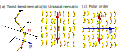
\includegraphics{\TwistBendFigures/Bananas.pdf}
    \caption{(a) The heliconical ground state of a twist-bend nematic, with director $\w n$ and shape polarisation $\w p$ of the banana shaped molecules shown. $\w p$ is parallel to the bend vector $\w b$ of the director. (b,c) Just as a uniaxial liquid crystal can exist in either an isotropic or nematic phase despite the individual molecules being rod-like, a banana shaped molecule does not automatically imply the twist-bend state --- these polar molecules may have their orientations randomly aligned to give no net shape polarisation, creating a uniaxial nematic phase. Figures reproduced from \citep{Lavrentovich2018}.}
    \label{fig:Bananas}
\end{figure}
\begin{equation}
    F_{\mathrm{tb}} =  \int d^3 {\bf r}\ \frac{K}{2}|\nabla {\bf n}|^2 +\frac{C}{2}|\nabla {\bf p}|^2 -\lambda \w p \cdot (\w n \cdot \nabla)\w n + \frac{u}{4}(1 - |\w p|^2)^2
    \label{eq:TwistBendFreeEnergy}
\end{equation}
where $K$ is a single Frank elastic constant for the director, $C$ is the same for the polarisation, $\lambda$ sets the strength of coupling between bend and polarisation, and $u$ sets the scale of the bulk ordering energy. One may coarse grain $\w p$ out of this free energy, reproducing Dozov's theory with an effective bend constant $K_3^{\mathrm{eff}} = K_3 - (2\lambda^2/u)$, which becomes negative if the ratio $\lambda^2/u$ is large enough \citep{Meyer2016}. The ground state of \eqref{eq:TwistBendFreeEnergy} appears to be given by \eqref{eq:TwistBendDirector}. Sending $u \rightarrow \infty$ in \eqref{eq:TwistBendFreeEnergy}, as is the case deep in the twist-bend phase, $|\w p|=1$ and $\w p$ is assumed to have the form  
\begin{equation}
\w p = (- \sin q z, \cos q z ,0).
\label{eq:TwistBendPolarisation}
\end{equation}
This limit is useful for theoretical intuition, although in all simulations of the free energy \eqref{eq:TwistBendFreeEnergy} presented in this chapter we allow the magnitude of $\w p$ to vary. Substituting the forms \eqref{eq:TwistBendDirector}, \eqref{eq:TwistBendPolarisation} into \eqref{eq:TwistBendFreeEnergy} one may determine the heliconical parameters in terms of those in the free energy,
\begin{align}
    \label{eq:theta}
    \cos 2 \theta &= \left( 1+ \frac{2C}{K} \right) - \left( \frac{4C}{K}  \left( 1+ \frac{C}{K} \right) \right)^\frac{1}{2},\\
    \label{eq:q}
    q &= \frac{2 \lambda}{K} \cot 2 \theta,
\end{align}
which may also be written
\begin{align}
    \frac{\lambda}{K} = \frac{q \tan 2 \theta}{2}, \quad 
    \frac{C}{K} = \frac{\sin^4\theta}{\cos 2 \theta}.
\end{align}
In terms of dimensionless variables $\lambda/K , C/K$ the magnitude of the heliconical bend is
\begin{align}
    |\w b| = q\sin\theta\cos\theta = \frac{\lambda}{K}\left( \left( 1+ \frac{2C}{K} \right) - \left( \frac{4C}{K}  \left( 1+ \frac{C}{K} \right) \right)^\frac{1}{2}\right).
    \label{eq:magb}
\end{align}
\begin{figure}[htbp]
    \centering
    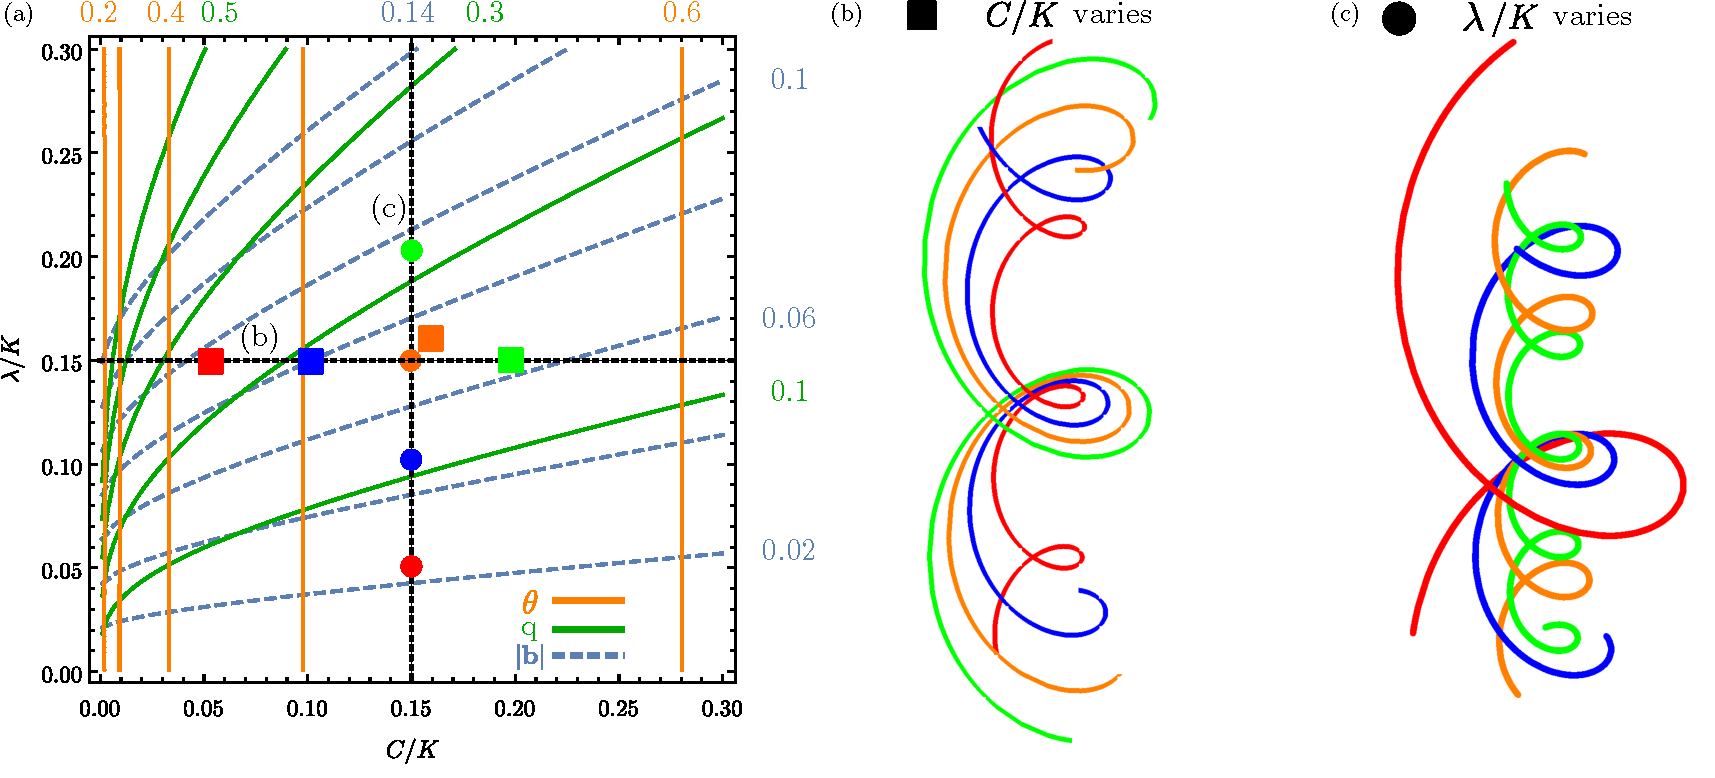
\includegraphics[width=\textwidth]{\TwistBendFigures/HeliconicalGroundState.pdf}
    \caption{(a) Contour plots of $\theta$ \eqref{eq:theta}, $q$ \eqref{eq:q} and $|b|$ \eqref{eq:magb} against $C/K, \lambda/K$ for the heliconical ground state \eqref{eq:TwistBendDirector} of the free energy \eqref{eq:TwistBendFreeEnergy}. Coloured squares and circles are particular values of $(C/K, \lambda /K)$ for which the corresponding integral curves of the director are shown in (b),(c).}
    \label{fig:HeliconicalGroundState}
\end{figure}
In figure \ref{fig:HeliconicalGroundState}(a) we plot $\theta, q, |\w b|$ as functions of $C/K, \lambda/K$. Fixing $\lambda/K$ and increasing $C/K$ causes the cone angle to increase towards an asymptotic value of $\pi/4$, and both wavevector and bend magnitude to decrease. Fixing $C/K$ and increasing $\lambda/K$ causes wavevector and bend magnitude to increase, with the cone angle unchanged. The integral curves of the director \eqref{eq:TwistBendDirector} are given by the helices
\begin{align}
    (x(t),y(t),z(t)) = (\frac{1}{q} \tan \theta \sin qt, \frac{1}{q} \tan \theta \cos qt,t),
\end{align}
and in figures \ref{fig:HeliconicalGroundState}(b),(c) we show the effects of varying $C/K, \lambda/K$ on these integral curves.

Theoretical prediction of the twist-bend nematic predated its experimental observation by decades \citep{Lavrentovich2018}, with optical microscopy experiments in the period $1993$--$2013$ suggesting the existence of a low temperature `$N_x$' state in a variety of flexible dimers, which supported focal conics as well as other hallmarks of a layered structure, but without an accompanying density wave (as in a smectic) and a periodicity too small to resolve (in contrast to a cholesteric). More direct observations came from freeze-fracture transmission electron microscopy in 2013 \citep{Borshch2013}, with an $N_{\mathrm{tb}}$ phase directly observed in cyanobiphenyl-$(\mathrm{CH}_2)_7$-cyanobiphenyl (CB$7$BC) with an extremely small pitch of $8$-$9$nm. Currently there are over $100$ compounds known to exhibit this phase, with prevailing pitch lengths on the nanometre scale \citep{Lavrentovich2018}. In comparison to cholesterics, with pitches in the $\mu m$, this certainly represents a current experimental difficulty in generating topologically nontrivial textures in these systems. 
\label{sec:GeometryTopologyOfBend}
\section{The structure of $\beta$ lines}
\label{sec:Structure}
Consider the 1-form $B := \langle b,b \rangle A$ and its dual vector $\w{B} := \langle B, \bullet \rangle$. The vector $\mathbf{j} := \nabla \times \mathbf{B}$ points along the $\beta$ lines, orienting them according to the circulation of $A$ as shown in figure~\ref{fig:BetaLines} \citep{Machon2016b}. To see this, consider a local trivialisation $(\w d_x, \w d_y,\w n)$ in a tubular neighbourhood around the $\beta$ line. Unlike $(\mathbf{b}, \mathbf{b}_\perp)$, $(\w d_x, \w d_y)$ are nonzero throughout the neighbourhood. In such a trivialisation, ${\bf b} = b_x \w{d}_x + b_y \w{d}_y,\ {\bf b}_\perp = b_x \w{d}_y - b_y \w{d}_x,\ \langle \w b, \w{b} \rangle = b_x^2 + b_y^2$. Expanding $A$ one finds
\begin{equation}
    A = \frac{b_x d b_y - b_y d b_x}{b_x^2 + b_y^2}+ \omega
    \label{eq:localA}
\end{equation}
where \omega := $\langle \w{d}_y, \nabla \w{d}_x \rangle$ is the connection $1$-form associated to $\nabla$ when using this local trivialisation. $(b_x,b_y,s)$, where $s$ is arclength along the $\beta$ line, form a local coordinate system with $z$-axis tangent to the $\beta$ line and given by $\nabla b_x \times \nabla b_y/|\nabla b_x \times \nabla b_y|$ --- generically $(b_x, b_y)$ vanish linearly, so $\nabla b_x, \nabla b_y$ are non-zero on the $\beta$ line and the coordinate system is well defined. We may also define the associated cylindrical polar system $(\rho,\theta,z)$\footnote{Remember, however, that the vectors $\nabla b_x/|\nabla b_x|$ and $\nabla b_y/|\nabla b_y|$ are not orthogonal and so there is a Jacobian between this and a `true' polar system.}, in which $A = d\theta + \omega$. The azimuthal 1-form $d\theta$ itself is undefined on the $\beta$ line, diverging relative to the smooth contribution $\omega$, and as such the essential behaviour of $A$ around the $\beta$ line is simply that of $d \theta$ (figure~\ref{fig:BetaLines}). Multiplying \eqref{eq:localA} through by $b_x^2 + b_y^2$, $\w{B} = b_x \nabla b_y - b_y \nabla b_x + (b_x^2 + b_y^2) \langle \omega, \bullet \rangle$  and on the $\beta$ line $\w{j} = \nabla \times \w{B} = 2 \nabla b_x \times \nabla b_y$. In terms of differential forms, on the $\beta$ line $dB = 2 d b_x \wedge d b_y$ and $\star dB$ is dual to $\w j$, where $\star$ denotes Hodge duality. We emphasise that $A$ and $d\theta$ are defined along the entire tubular neighbourhood of a generic $\beta$ line (with the line itself cut out), providing a canonical orientation.
\begin{figure}[htbp]
    \centering
    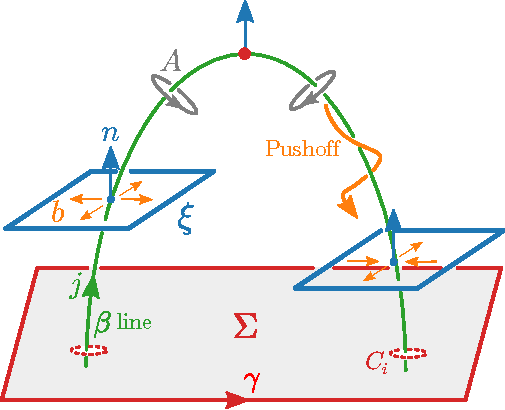
\includegraphics[keepaspectration, width=0.7\linewidth ]{\TwistBendFigures/BetaLine6.pdf}
    \caption{The bend $\w n$ (orange arrows), a section of the bundle of planes $\xi$ (blue planes) which are perpendicular to the director $\w n$ (blue arrows), vanishes along curves called $\beta$ lines (green curve). The 1-form $A$ \eqref{eq:1form} (grey) circulates around these $\beta$ lines, providing a global orientation vector $\w j$. The figure shows a Legendrian point in the $\beta$ line (red dot), where $\w n \cdot \w j =0$, and across which the index of the $\beta$ line $I_\beta^\xi$, which characterises its local profile, changes.}
    \label{fig:BetaLines}
\end{figure}

\subsection{The local structure of $\beta$ lines}
\label{subsec:LocalStructure}
We may investigate the local structure of $\w b$ about a $\beta$ line via a Taylor series. Generically this series is governed by linear terms and so its structure is given by $\nabla \w b$ evaluated on the $\beta$ line. We have already seen that the director $\w n$ splits $T \mathbb{R}^3\approx L \oplus \xi$, with a corresponding splitting of $\nabla \w n$ into two pieces, $\nabla^L \w n $ and $\nabla^\xi \w n$, in \S\ref{subsec:Geometry}, and one way to proceed is to do same to $\nabla \w b$. However, the $\beta$ line itself, in combination with $\w n$ along it, provides us with more structure than a single splitting --- it gives a canonical way to further split $\xi$, giving an adapted framing with which several other planes and splittings may then be defined. In figure \ref{fig:Splittings}(a) we show the $\beta$ line and $\w n$ at a generic point, where $\w n$ and $\w j$ are neither parallel nor perpendicular. The normalised cross product $\w n \times \w j$ defines a vector $\w n_\lambda := \w n \times \w j/| \w n \times \w j|$ and orthogonal plane $\lambda$, and we define a third vector $\w n_\chi := \w n_\lambda \times \w n = (\w j - (\w n\cdot \w j)\w n)/|\w j - (\w n\cdot \w j)\w n|$, the normalised projection of $\w j$ onto $\xi$, with associated orthogonal plane $\chi$. Setting $(\w d_x, \w d_y, \w n) = (\w n_\chi, \w n_\lambda, \w n)$ gives an adapted frame for the $\beta$ line, with the line itself always in the $\lambda$ plane. Note immediately that by construction, $\w n_\chi \cdot \w j \geq 0$, and further that this frame is undefined if $\w n \parallel \w j$. Across such points both $\w n_\chi$ and $\w n_\lambda$ change sign discontinuously, and the framing undergoes a $\pi$ rotation (as unoriented planes $\chi$ and $\lambda$ may be extended by continuity) --- this situation is shown in figure  \ref{fig:Splittings}(b), and we shall return to it in a moment. As well as $\xi, \chi$ and $\lambda$, we also have the plane perpendicular to $\w j$ itself, given by $\mathrm{ker}(\star dB)$ and denoted $\alpha$. Loops in these planes measure winding about the $\beta$ line. We have two limiting cases, shown in figures \ref{fig:Splittings}(b) and (c). In figure~\ref{fig:Splittings}(b), $\w  n \parallel \w j$, $\xi = \alpha$ and a loop in $\chi$ intersects the $\beta$ line --- if we try to measure winding on this plane we encounter degenerate behaviour. In figure~\ref{fig:Splittings}(c) $\w n \perp \w j$, $\chi = \alpha$ and a loop in $\xi$  intersects the $\beta$ line, likewise showing degenerate behaviour. This latter case, where $\w n \cdot \w j= 0$, we refer to as a Legendrian point \citep{Geiges2009}. One notes that the degeneracy in figure \ref{fig:Splittings}(b) is of higher codimension than that in figure \ref{fig:Splittings}(c) --- in figure \ref{fig:Splittings}(c) we require one component of a unit vector to vanish, giving a codimension $1$ degeneracy, whereas in figure \ref{fig:Splittings} two must vanish, giving codimension $2$.
\begin{figure}[htbp]
    \centering
    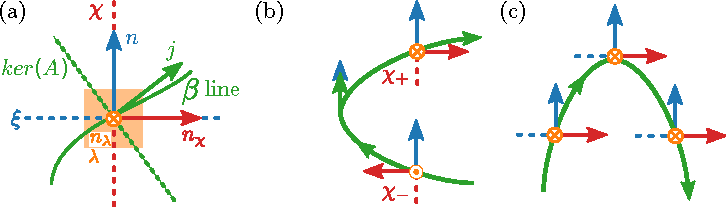
\includegraphics[keepaspectration, width=0.99\linewidth ]{\TwistBendFigures/Splittings.pdf}
    \caption{(a) At a generic point on a $\beta$ line we have a canonically defined triple $(\w n_\chi, \w n_\lambda, \w n)$ with orthogonal planes $(\chi,\lambda, \xi)$, as well as the tangent to the $\beta$ line $\w j$ and its orthogonal plane $\alpha$. This framing breaks down in the situation shown in panel (b), where  $\w n \parallel \w j$ and $\w n_\lambda$ is undefined, a codimension $2$ degeneracy. In (c) we show a Legendrian point where $\w n \cdot \w j = 0$, a codimension $1$ degeneracy. Measuring on a consistently oriented plane across these degeneracies (in other words using either $\chi_-$ or $\chi_+$ across the degeneracy in (b)), in (b) $I^\chi_\beta$ changes sign and in (c) $I^\xi_\beta$ changes sign.}
    \label{fig:Splittings}
\end{figure}

We now examine the structure of $\nabla \w b$ on the $\beta$ line, making use of the various planes defined above. In general, $\nabla \w b \in \Gamma(T^*\mathbb{R}^3 \otimes T\mathbb{R}^3)$. Note, however, that $\langle \w n, \nabla \w b \rangle = - \langle \w b , \nabla \w n \rangle$ and so along a $\beta$ line, where $\w b=0$, $\nabla \w b$ takes values in $T^*\mathbb{R}^3 \otimes \xi$ and so can be viewed as a linear map $\mathbb{R}^3 \rightarrow \mathbb{R}^2$, with a one-dimensional kernel which defines the $\beta$ line; $\w j$ lies in this kernel. We have that 
\begin{equation}
    \w j = \mathrm{det}(\nabla^{\alpha} \w b) \hat{\w j} = \mathrm{det}(\nabla^\xi \w b) \w n + \mathrm{det}(\nabla^\chi \w b) \w n_\chi
\label{eq:IndexRelation}
\end{equation}
where, as defined in \S{\ref{subsec:Geometry}}, $\nabla^\bullet \w b$ is the restriction of $\nabla \w b \in \Gamma(T^*\mathbb{R}^3 \otimes \xi) $ to the space $\bullet^* \otimes \xi$. It is understood that each $\nabla^\bullet \w b$ is evaluated on the $\beta$ line, and one may imagine each reads $\nabla^\bullet \w b |_{\beta\ \mathrm{line}}$ although we shall not explicitly write the restriction. Each equality in \eqref{eq:IndexRelation} is just a rewriting of the cross product $\nabla b_x \times \nabla b_y$, but they may be obtained directly by pulling back the volume form on $\xi$ via $\nabla \w b$. Using the second equality  in \eqref{eq:IndexRelation} as an example, we have the decomposition $\nabla \w b = \nabla^\xi \w b E_\xi + \nabla^\chi \w b E_\chi+ \nabla^\lambda \w b E_\lambda$, where $E_\bullet$ denotes projection onto the subspace $\bullet$ as in \S{\ref{subsec:Geometry}. This decomposition carries through to the pullback, and since each of $\nabla^\xi \w b , \nabla^\chi \w b,\nabla^\lambda \w b $ is a map between vector spaces of the same dimension, the pullback simply scales the volume form by the determinant. Finally, by the construction of our framing, $\mathrm{det}(\nabla^\lambda \w b) =0$ --- if we were using an arbitrary framing all three terms would appear in \eqref{eq:IndexRelation}. Recall also that, by the construction of $\w n_\chi$, $\det\nabla^\chi \w b \geq 0$.

 \eqref{eq:IndexRelation} relates the windings we see in different measuring loops around the $\beta$ line, and allows us to examine winding behaviour as we pass through a Legendrian point. In the above discussion we focused on $\xi$ and $\chi$, but it is worth also describing what one observes when measuring winding on a general oriented plane $\gamma$. Pairing a unit vector in $\mathbb{R}^3$ to its orthogonal oriented plane, the space of all such planes is $S^2$, and we imagine $\w j $ defining a north pole. The set of all planes containing the $\beta$ line is then an equatorial circle which splits $S^2$ into two disconnected hemispheres --- in passing from one piece to another we encounter a plane containing the $\beta$ line, on which $\mathrm{det}(\nabla^\gamma \w b) = 0$ and across which it changes sign. This description motivates the definition of an index $ I^\gamma_\beta := \mathrm{Sgn}(\mathrm{det}(\nabla^\gamma \w b)) =\mathrm{Sgn}(\w n_\gamma \cdot \w j)$, where $\w n_\gamma$ is the unit vector associated with the oriented plane $\gamma$. The most common measurement of this type is $I^\xi_\beta$ \citep{Nye1987,Berry1998,Berry2004}, which describes the winding of $\w b$ measured on a loop in the oriented plane $\xi$. The value of $I^\gamma_\beta$ depends on which of the two equivalence classes outlined above $\gamma$ belongs to; if $\gamma$ is degenerate and $\mathrm{det}(\nabla^\gamma \w b)=0$, we set $I^\gamma_\beta=0$. By construction, $I^\lambda_\beta=0$, $I^\chi_\beta= \{0,1\}$. This latter fact is a little subtle given the reversal of $\w n_\chi$ when $\w n \parallel \w j$; we return to it in a moment.  

 Let us now consider situations of degeneracy in order of ascending codimension, beginning with a Legendrian point (codimension $1$), shown in figure~\ref{fig:Splittings}(c) and also in figure~\ref{fig:BetaLines}. At the point itself $\w n \cdot \w j =0$ so $I^\xi_\beta=0$ and we encounter degenerate winding on $\xi$; across the point $I^\xi_\beta$ changes sign. By contrast, the winding measured in $\alpha = \chi$, given by $I^{\chi}_\beta$, is perfectly well behaved. The dual situation (codimension $2$) occurs when $\w n \cdot \w j = \pm 1$, $I^\chi_\beta=0$ and is shown in figure \ref{fig:Splittings}(b). Across such points, the orientation of $\chi$ reverses. To be precise let us define a $+$ and $-$ side of the point, with associated oriented planes $\chi_+$ and $\chi_-$ which may be smoothly continued across the singular point and so defined on a neighbourhood of it. On the $+$ side $I^\chi_\beta = I_\beta^{\chi_+}$, and on the $-$ side $I_{\beta}^\chi = I_{\beta}^{\chi_-}$. We have that $I_{\beta}^{\chi_+} = -I_{\beta}^{\chi_-}$ and so measurement of index on a consistently oriented plane across the singular point shows a sign reversal. Finally $\mathrm{det}(\nabla^{\alpha}\w b)^2 = \mathrm{det}(\nabla^\xi \w b)^2+ \mathrm{det}(\nabla^\chi \w b)^2$, and so for $I^{\mathrm{\alpha}}_\beta$ to vanish we require that $I^\xi_\beta = I^\chi_\beta = I^\lambda_\beta=0$, in other words that $\w j$ vanish, an even higher codimension degeneracy in which $\mathrm{ker}(\nabla \w b)$ become two-dimensional and the coordinate system $(b_x,b_y)$ defined above breaks down. 

We briefly explore how these constructions appear when given a concrete, but arbitrary, trivialisation $(\w d_x,\w d_y,\w n)$. With respect to this trivialisation $\nabla \w b$ is given a $2\times3$ matrix and we have a Taylor series
\begin{align}
\begin{pmatrix}b_x \\ b_y\end{pmatrix} = 
\begin{pmatrix} 
    \nabla^\xi \w b_{xx} & \nabla^\xi \w b_{xy} & s_{xz}\\
    \nabla^\xi \w b_{yx} & \nabla^\xi \w b_{yy} & s_{yz}\\ 
\end{pmatrix}
\begin{pmatrix}x \\ y \\ z \end{pmatrix}  
+ O(2)
\label{eq:gradbmatrix}
\end{align}
where $s_{xz},s_{yz}$ are currently regarded simply as undetermined constants in the Taylor series. How should we extract the adapted frame, orientation of the $\beta$ line and local windings from this matrix? $I_\beta^\xi$ is immediate. $\w j$ is given by
\begin{align}
    \w j &= (\nabla^\xi \w b_{xy}s_{yz} - \nabla^\xi \w b_{yy}s_{xz})\w d_x -( \nabla^\xi \w b_{xx}s_{yz} - \nabla^\xi \w b_{yx}s_{xz})\w d_y + \mathrm{det}(\nabla^\xi \w b) \w n \\
         &= \mathrm{det}(\nabla^{\chi^{'}} \w b)\w d_x  -\mathrm{det}(\nabla^{\lambda^{'}} \w b)\w d_y + \mathrm{det}(\nabla^\xi \w b) \w n = \mathrm{det}(\nabla^{\chi}\w b)\w n_\chi + \mathrm{det}(\nabla^\xi \w b) \w n
\end{align}
where $\chi'$ and $\lambda'$ are the planes associated to the unadapted frame $(\w d_x,\w d_y, \w n)$. We have that $\mathrm{det}(\nabla^{\chi} \w b)= (\mathrm{det}(\nabla^{\lambda^{'}} \w b)^2 + \mathrm{det}(\nabla^{\chi'}\w b)^2)^\frac{1}{2}$, where we may safely choose the positive branch of the square root by construction of $\w n_\chi$. Away from a Legendrian point $\w{j}$ may also be written as $\w j = \mathrm{det}(\nabla^\xi \w b)(\nabla^\xi \w b^{-1}\w{s},1)^T$, where $\w s = (s_{xz}, s_{yz})^T$, and so the orientation on the $\beta$ line is determined by $\nabla^\xi \w b^{-1} \w s$ --- specifically, its angle to the local $z$-axis is given by $\tan\theta = \mathrm{det}(\nabla^{\chi}\w b)/ \mathrm{det}(\nabla^{\xi}\w b)= \w s^T (\nabla^\xi \w b^{-1})^T \nabla^\xi \w b^{-1} \w s$, and to the $x$-axis by $\cos \phi =\mathrm{det}(\nabla^{\chi'}\w b) /\mathrm{det}(\nabla^{\chi}\w b)$ --- a rotation by $\phi$ adapts the framing, bringing $\chi'=\chi, \lambda' = \lambda$, at which point \eqref{eq:gradbmatrix} adopts the form
\begin{align}
\begin{pmatrix}b_x \\ b_y\end{pmatrix} = 
\begin{pmatrix} 
     \cot \theta s_{xz}& \nabla^\xi \w b_{xy} &s_{xz}\\
    \cot \theta s_{yz}& \nabla^\xi \w b_{yy} & s_{yz}\\ 
\end{pmatrix}
\begin{pmatrix}x \\ y \\ z \end{pmatrix}  
+O(2)
\label{eq:gradbmatrix}
\end{align}
where $\nabla^\xi \w b_{xy}$ etc. now refer to the rotated coordinate values. At a Legendrian point, $\mathrm{det}(\nabla^\xi \w b)=0$, but \eqref{eq:gradbmatrix} and our expression for $\cos \phi$ still holds in the limit $\theta \rightarrow \pi/2, \cot \theta \rightarrow 0$. The limit where $\theta \rightarrow 0$ is a little more delicate. Here $s_{xz}, s_{yz} \rightarrow 0$, and one needs to prescribe a manner in which they do so in order to find the limiting framing behaviour --- for example, $\cos\phi = (1+(\mathrm{det}\nabla^\lambda' \w b)^2 /(\mathrm{det}\nabla^\lambda' \w b)^2)^{-\frac{1}{2}} = (1+ (\nabla^\xi \w b_{xx} s_{xz} - \nabla^\xi \w b_{yx} s_{yz})^2/(\nabla^\xi \w b_{yx}s_{xz}-\nabla^\xi \w b_{yy} s_{yz})^2)^{-\frac{1}{2}}$, and this expression can give arbitrary values of $\phi$ depending on how the limits in $s_{xz}, s_{yz}$ occur.
\subsection{Relating $\beta$ line structure to director gradients}
\label{subsec:RelatingtoDirector}
 Above, we studied the structure of $\nabla \w b$ on $\beta$ lines and the possible local structures of bend around them. All of this structure is derived from that of $\w n$, and it is interesting to investigate their correspondence. For example, it is relatively easy to imagine a director field which gives a bend zero with index $I^\xi_\beta=+1$: we picture $\w n$ tangent to a family of helices all centred on a local axis, their radius decreasing as one approaches the axis and degenerating to a line along the axis itself. A director with $I^\xi_\beta=-1$ is perhaps less obvious; how should we construct and visualise one?  Further, as noted above, this family of helices has the director parallel to the $\beta$ line, a highly nongeneric, codimension $2$, situation: what is the generic one?

We begin by relating the bend structure about a $\beta$ line to director gradients: a direct calculation yields $\nabla^\xi \w{b} = (\nabla^\xi{\bf n})^2+\nabla^L \nabla^\xi{\bf n}$ , $\nabla^L \w b = (\nabla^L)^2 \w n$. With respect to an arbitrary $(\w d_x,\w d_y, \w n)$ trivialisation the corresponding Taylor series for the director, retaining only terms that contribute to the bend at linear order, is
\begin{align}
\begin{pmatrix} n_x \\ n_y \end{pmatrix} & = \biggl( \nabla^\xi {\bf n}  + z  \nabla^L\nabla^\xi {\bf n} \biggr) \begin{pmatrix} x \\ y \end{pmatrix} + \frac{1}{2} z^2 \begin{pmatrix} (\nabla^L)^2 n_x \\ (\nabla^L)^2 n_y \end{pmatrix}
\label{eq:DirectorTaylor}
\end{align}
giving bend
\begin{align}
\begin{pmatrix}b_x \\ b_y\end{pmatrix} & =
\biggl(\left(\nabla^\xi {\bf n}\right)^2+ \nabla^L\nabla^\xi {\bf n} \biggr) \begin{pmatrix} x \\ y \end{pmatrix}
 + z \begin{pmatrix}(\nabla^L)^2 n_x \\ (\nabla^L)^2 n_y \end{pmatrix},
\label{eq:BendTaylor}
\end{align}
which may then be cast into the form of \eqref{eq:gradbmatrix}. We emphasise again that all operators in \eqref{eq:DirectorTaylor}, \eqref{eq:BendTaylor} are evaluated on the $\beta$ line. Pursuing our investigation of zeros of differing index we decompose $\nabla^\xi \w{b}$ into two components, a spin 0 component $\nabla^{\xi, +} \w{b}$ with positive determinant and winding, and a spin 2 component $\nabla^{\xi, -} \w{b}$ with negative determinant and winding: $\nabla^\xi \w{b} = \nabla^{\xi,+} \w{b} + \nabla^{\xi,-} \w{b}$. With this decomposition one finds that $\w{n} \cdot \w{j} = \mathrm{det}(\nabla^\xi \w{b}) = |\mathrm{det}(\nabla^{\xi, +} \w{b})| - |\mathrm{det}(\nabla^{\xi, -} \w{b})| $ and so the relative weights of each component determine the overall index. $\nabla^{\xi,+} \w{b}$, $\nabla^{\xi,-} \w{b}$ may again be explicitly computed in terms of the director by recalling the splitting of the shape operator~\eqref{eq:GradientDecompositionperp}
\begin{align}
    \nabla^\xi {\bf n}= \frac{s}{2}I_\xi + \frac{q}{2} J + \Delta
\end{align} 
where $s = \nabla \cdot \w n$ is the splay, $q = \w n \cdot \nabla \times \w n$ is the twist, and $\Delta$ is the deviatoric component~\citep{Machon2016b,AlexanderBook,Selinger2019}, all evaluated on the $\beta$ line. We find that
\begin{align}
\nabla^{\xi,+} \w{b} &=
\frac{1}{4}\Big(s^2 - q^2 - 4\mathrm{det}\Delta +2\nabla_{\w n} s\Big)I_\xi+
\frac{1}{2} \Big(sq + \nabla_{\w n} q \Big)J,  \\
\nabla^{\xi,-} \w{b} &= s \Delta +\nabla_{\w n} \Delta.
\end{align}
Note that in the absence of variation along $\w n$, $\nabla^\xi \w{b} = (\nabla^\xi{\bf n})^2$ and only an index of $I^\xi_\beta = +1$ is possible; for negative winding we must have nonzero derivatives along the director.

$\nabla_{\w n} \Delta$ itself is naturally decomposed into two modes of distortion --- change in the magnitude of the eigenvectors of $\Delta$, and their rotation:
\begin{align}
    \nabla \Delta = \frac{\langle \Delta, \nabla \Delta \rangle}{\langle \Delta, \Delta \rangle}\Delta + \frac{\langle \Pi, \nabla \Delta \rangle}{\langle \Delta, \Delta \rangle} \Pi,
\end{align}
where $\Pi = J \Delta$ is orthogonal to $\Delta$ with respect to the inner product, $\langle \Pi ,\Delta \rangle = \mathrm{Tr}(\Pi^\dagger \Delta) = 0$. The object $\frac{\langle \Pi, \nabla \Delta \rangle}{\langle \Delta, \Delta \rangle}$ is a connection 1-form defined in Ref.~\cite{Machon2016b}, which measures the rotation of $\Delta$. To see this explicitly, consider $\Delta$ expressed in a $(\w d_x, \w d_y, \w n)$ trivialisation, 
\begin{align}
    \Delta = 
    \begin{pmatrix}
        \Delta_1 & \Delta_2 \\
        \Delta_2 & -\Delta_1
    \end{pmatrix}
    = \sqrt{-\mathrm{det}\Delta}
    \begin{pmatrix}
        \cos \theta & \sin \theta \\
        \sin \theta & -\cos \theta
    \end{pmatrix}
\end{align}
Direct calculation shows that $\frac{\langle \Pi, \nabla_{\w n} \Delta \rangle}{\langle \Delta, \Delta \rangle} = d\theta(\w n) + 2 \langle \w d_y, \nabla_{\w n} \w d_x \rangle$. The second term expresses the rotation of $(\w d_x,\w d_y)$ as one moves along $\w n$, and we may set it to $0$ by demanding that the trivialisation to be locally parallel (the closest we can come to demanding it be constant given that $\xi$ varies). Then  $\frac{\langle \Pi, \nabla_{\w n} \Delta \rangle}{\langle \Delta, \Delta \rangle} = d\theta(\w n) = \theta'$. With this notation in hand
\begin{multline}
 \mathrm{det}(\nabla^\xi \w{b}) =
 \left( (s/2)^2 +(q/2)^2 +\mathrm{det}\Delta\right)^2 \\
+ (\nabla_{\w n} s/2)^2+(\nabla_{\w n} q/2)^2
+ \left((s/2)^2-(q/2)^2)\nabla_{\w n} s
+ \left(sq/2\right) \nabla_{\w n} q \\
+ s(\nabla_{\w n} \mathrm{det}\Delta) -\mathrm{det}\Delta\right)\nabla_{\w n} s - \left(\nabla_{\w n} \sqrt{-\mathrm{det} \Delta}\right)^2 + \mathrm{det}\Delta \theta'^2.
    \label{eq:nablabdeterminant}
\end{multline}
Note that setting all gradients to $0$ in \eqref{eq:nablabdeterminant} we recover $\mathrm{det}(\nabla^\xi \w n)^2$, whilst setting all terms involving $\Delta$ to 0 we recover $\mathrm{det}( \nabla^{\xi,+} \w b)$.

 In figure \ref{fig:BendZeros}(a) we show director and bend configurations for each mode of distortion appearing in \eqref{eq:nablabdeterminant}. In figure \ref{fig:BendZeros}(b) we show a succession of profiles one might see in crossing a Legendrian point, for example following the $\beta$ line in figure \ref{fig:BetaLines} --- in the example shown $\theta'$ increases, changing an $I_\beta^\xi=+1$ profile to an $I_\beta^\xi=-1$ profile, with a corresponding change in the sign of $\w n \cdot \w j$. 
\begin{figure}[htbp]
    \centering
    \includegraphics[keepaspectration, width=\linewidth ]{\TwistBendFigures/BendZeros.pdf}
    \caption{(a) Each mode of distortion appearing in \eqref{eq:nablabdeterminant}, with corresponding bend zero. In all but the last panel, only the given mode is nonzero. In the last panel, both $\mathrm{det \Delta}$ and $\theta'$ are nonzero --- one needs principal axes defined to see their twisting. $\w j$ is shown aligned with the director, although we emphasise this is nongeneric. (b) With $\mathrm{det\Delta}$ initially nonzero and all other modes zero, $\theta'$ is increased, giving a series of profiles one might see in crossing a Legendrian point. In the figure the skew of the $\beta$ line relative to $\xi$ is set to a generic nonzero value --- note the sign change in $\w n \cdot \w j$ with that of $I_\beta^\xi$.}
    \label{fig:BendZeros}
\end{figure}

\subsection{Self-Linking of $\beta$ lines}
\label{subsec:Self-Linking}
As we follow a closed $\beta$ line, the local structure described in \S\ref{subsec:LocalStructure}, \ref{subsec:RelatingtoDirector} varies, providing a natural definition of self-linking --- the description we provide here is entirely analogous to that given for umbilic lines in Ref. \citep{Machon2016b}. Variation in local profile is tracked by measuring $\nabla^\xi \w b$ along the $\beta$ line (one might consider a different plane, $\alpha$ for example, but the results of the construction will not differ). At a fixed point on the $\beta$ line, the space of values of $\nabla^\xi \w b$ is described by four parameters, which cannot all be zero, and as such has the homotopy type of $S^3$. To compare $\nabla^\xi \w b$ at differing points along the $\beta$ line we introduce a local trivialisation of the bundle $\xi^*\otimes\xi$, for which a natural choice is induced by two sections $(d_x,d_y)$ of $\xi$ which have self-linking number $0$ with the $\beta$ line--- these may be explicitly constructed using the Solid Angle framing of \S\ref{ch:Maxwell}. Relative to this framing $\nabla^\xi \w b$ is a map from $S^1 \rightarrow S^3$. Such a map is nullhomotopic, and so to define a winding number we must impose some further restriction on the space of local profiles. A natural one is to restrict $I_\beta^\xi$ to a single sign, considering a transverse $\beta$ line with no Legendrian points. $S^3$ is then split into two solid tori \citep{Machon2016b}, and $\nabla^\xi \w b$ is homotopic to a map $S^1 \rightarrow S^1$ --- the degree of this map defines a longitudinal winding number. Suppose for definiteness we are in the solid torus such that $I^\xi_\beta= +1$. Given the splitting $\nabla^\xi \w b =  \nabla^{\xi,+}\w b +\nabla^{\xi,-}\w b$, this homotopy consists of tuning the term $\nabla^{\xi,-}\w b$ to zero, leaving only $\nabla^{\xi,+}\w b$ which is parameterised by two numbers, both nonzero, homotopically $S^1$.

If $\nabla^\xi \w b$ describes a `twisted tube' along the $\beta$ line, we may extract a ribbon by evaluating it on one of the trivialising sections, $\w d_x$ say, producing the vector field $\nabla^\xi_{\w d_x} \w b$ along the $\beta$ line whose self-linking number $\mathrm{SL}(\beta)$ equals the winding number described above. Such a ribbon is shown schematically in figure \ref{fig:BetaLines} and we shall see several examples in twist-bend nematics in \ref{sec:TopologicalSignificance}.
 
\section{The Topological Significance of $\beta$ lines}
\label{sec:TopologicalSignificance}

In \S \ref{sec:Elements},\ref{sec:Structure} we explored the structure of bend, and in particular its zeros, $\beta$ lines. In this section we shall see how these structures convey global topological information about the director $\w n$, with examples provided of Skyrmions and Hopfions in twist-bend nematics.  

\subsection{$\beta$ lines and Skyrmions}

Consider a measuring surface $\Sigma$ with boundary $\gamma$ inside $M$, with small disks of boundary $C_i$ removed where the $\beta$ lines puncture this surface, as shown in figure \ref{fig:BetaLines}. Integrating $A$ over this surface, by an analysis identical to that presented for umbilics in Ref.~\cite{Machon2016b} we have a result in the style of the Gauss-Bonnet-Chern theorem\citep{Lee1996,Frankel2015}:
\begin{equation}
    \frac{1}{2\pi}\int_\gamma A - \frac{1}{2\pi}\int_\Sigma \Omega = \frac{1}{2\pi}\sum_i \int_{C_i} d \theta = \sum_i \mathrm{Sgn}(\w n_{\Sigma} \cdot \w j) = \sum_i I_\beta^{C_i},
    \label{eq:GaussBonnetChern}
\end{equation}
where $I_\beta^{C_i}$ is the index of the $\beta$ line measured on the oriented plane containing $C_i$, dual to the $\w n_\Sigma$, the surface normal to $\Sigma$; $I_\beta^{C_i}$ may be $\pm I_\beta^\xi$. Suppose now that $\Sigma$ is closed. On this surface, the degree of the map $\w n : \Sigma \rightarrow  S^2$ counts the number of Skyrmions $q$, as discussed in\S\ref{subsec:SkyrmionsAndHopfions}. This degree may alternately be computed via the integral $1/4\pi \int_\Sigma \Omega$ \citep{Frankel2015}, and thus we have that $\sum_i I_\beta^{C_i}=2q$ --- a signed count of $\beta$ lines computes (twice the) Skyrmion number, and a nonzero Skyrmion number implies the existence of $\beta$ lines. In the language of characteristic classes \citep{MilnorStasheffBook} a closed set of oriented $\beta$ lines is a cycle in $H^1(M)$, Poincar\'{e} dual to the Euler class of $\xi$, $e(\xi)\in H^2(M)$. When we count signed intersections of this cycle with closed measuring surfaces, we are evaluating $e(\xi)$ on homology cycles in $H_2(M)$, producing characteristic numbers --- here the Euler characteristic. These numbers provide information --- here complete information \citep{MilnorStasheffBook} --- about whether the bundle is trivial or not.
\begin{figure}[htbp]
    \centering
    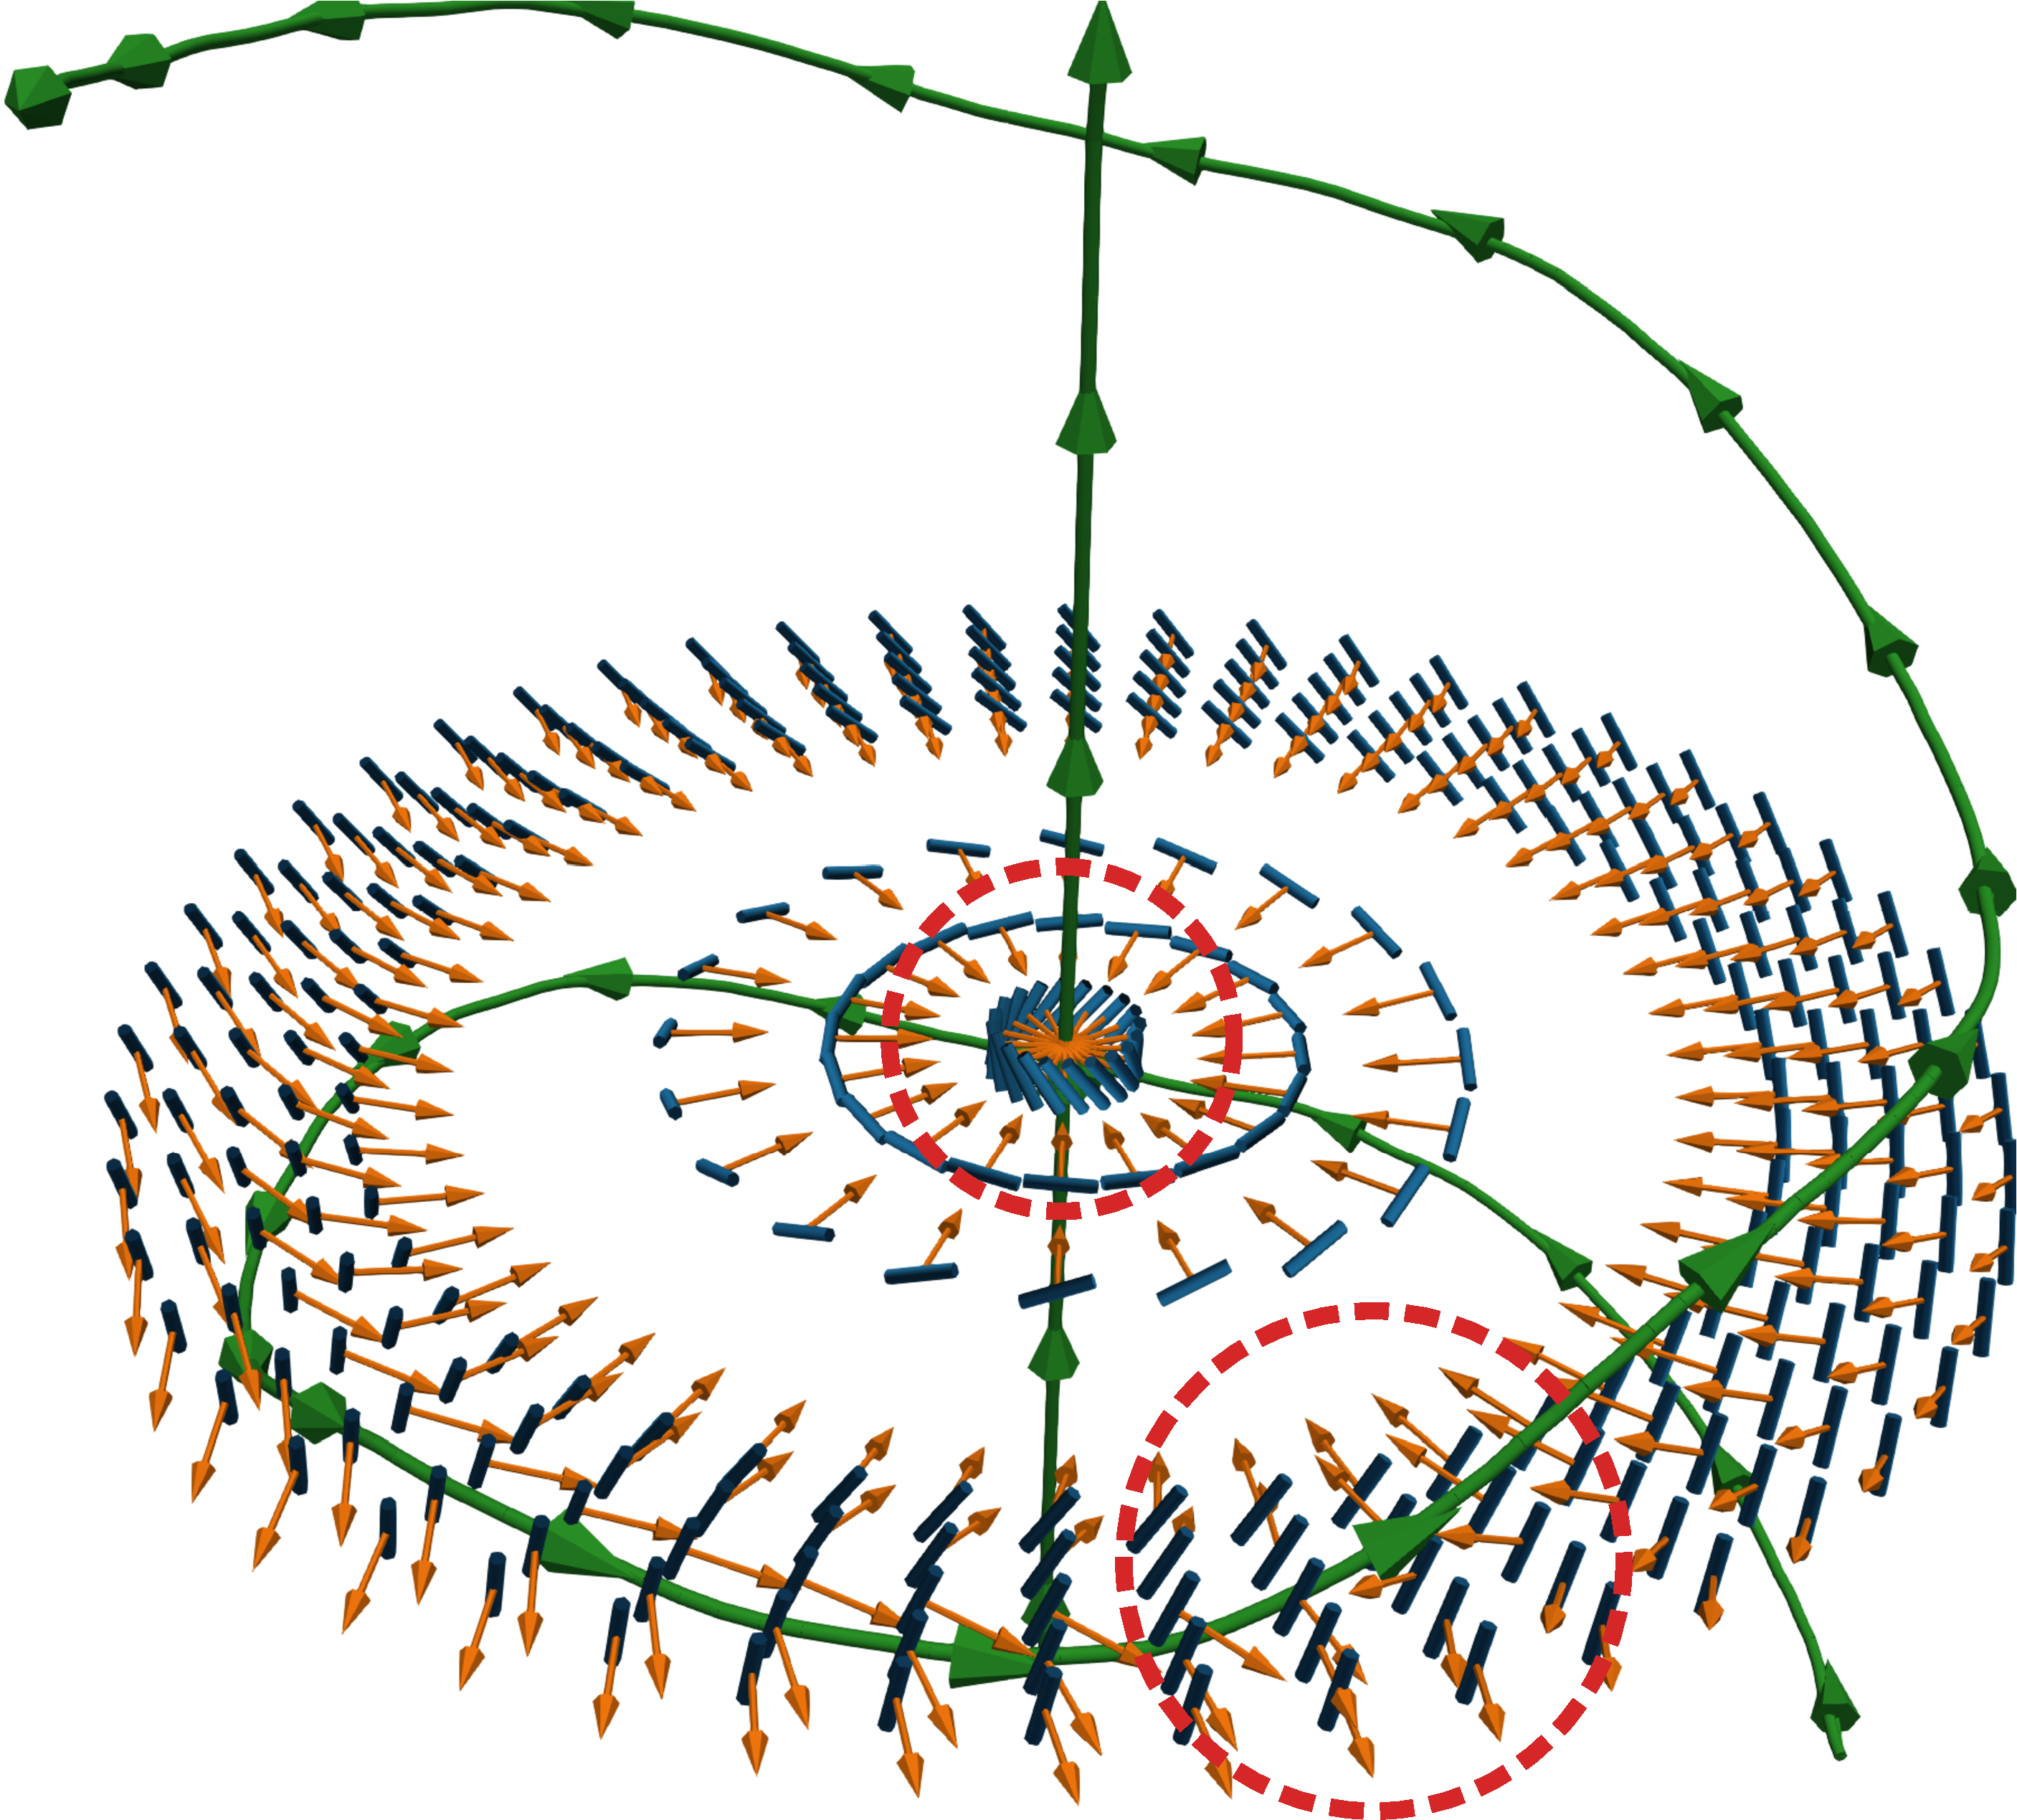
\includegraphics[width=0.5\textwidth]{\TwistBendFigures/TwistBendSkyrmion_annotated.pdf}
    \caption{Skyrmion tube in a twist-bend nematic, with $\beta$ lines oriented by $\w j$ shown in green, and a cross section through the tube, which may be taken as a measuring surface, containing director (blue cylinders) and normalised bend vector (orange arrows). A signed intersection count of the $\beta$ lines piercing this surface gives $+2$, twice the skyrmion number, consistent with \eqref{eq:GaussBonnetChern} --- these intersection points are highlighted in red circles, within which we see winding of the bend vector about its zeros.}
    \label{fig:TwistBendSkyrmion}
\end{figure}

In figure \ref{fig:TwistBendSkyrmion} we show a simulation of a skyrmion tube in a twist-bend nematic, with director and bend shown on a single cross section through the tube, which may be taken as our surface $\Sigma$. The texture tends to the heliconical ground state \ref{eq:TwistBendDirector}, \ref{eq:TwistBendPolarisation} in the far field, and so on a cross section we see a constant far field director and bend vector --- these rotate as the cross section is varied along the tube. This far field behaviour allows us to compactify the boundary of $\Sigma$ as is usual when measuring Skyrmion number, considering it closed as in the discussion above. We see that our Skyrmion texture is punctured by two bend zeros, both positively co-oriented with the surface, giving a count of $+2$, twice the Skyrmion number, and telling us that the bundle $\xi$ has nontrivial Euler class. Note that summing $I^\xi_\beta$ gives $1-1=0$, a reflection of the fact that the director makes a half twist between the two zeros. We briefly note that the $\beta$ lines are consistently transverse to the director (although the central $\beta$ line is nongeneric), and that their handedness is in fact opposite to that of the director, both observations deserving of further study.

\subsection{$\beta$ lines and Hopfions}

In \ref{subsec:SkyrmionsAndHopfions} we gave an introduction to Hopfions, three dimensional analogues of Skyrmions characterised by an element $Q$ of $\pi_3(S^2)$ for an orientable director --- we described how they may be visualised using the Pontryagin-Thom construction, and provided experimental images of their realisation in cholesterics. It has been suggested that their stability in cholesterics (escaping Derrick's theorem) comes from the intrinsic lengthscale in the ground state given by the repeat length $\pi/q_0$ \citep{Ackerman2017}. This motivates their study in twist-bend nematics, which have a similar ground state and lengthscale \eqref{eq:q}. Hopfions are also the ideal test case for probing what topological information $\beta$ lines contain in addition to the Euler class $e(\xi)$. More specifically, all three manifolds are parallelisable \citep{Geiges2009}, and once a choice of basis has been made the director gives a map $\w n :M\rightarrow S^2$. The homotopy class of such a map is determined firstly by the Euler class $e(\xi)$ and secondly by a suitably defined element of $\pi_3(S^2)$. In a Hopfion $M=S^3$ and so $H^2(M)$, hence $e(\xi)\in H^2(M)$, is zero. Can the $\beta$ lines tell us the Hopf invariant $Q$, the only topological information left, of the director?

In figure \ref{fig:Hopf} we show a Hopfion in a twist-bend nematic, simulated using a standard finite difference relaxation scheme applied to \eqref{eq:TwistBendFreeEnergy}, with fixed boundary conditions top and bottom and periodic boundaries in the horizontal plane, as is commonly used when simulating cholesteric Hopfions under confinement \citep{Ackerman2017}. In the vertical the simulation box is $2(2\pi/q)$, in the horizontal $8(2\pi/q)$. The texture itself is visualised using the Pontryagin Thom construction of \ref{subsec:HomotopyTheory} applied to the director. There are multiple constructions which explicitly realise such textures--- in the figure we simply rotate a skyrmion texture around a central axis as described in \citep{Sutcliffe2007}, giving a Hopfion with Hopf charge $Q=+1$, with the polarisation field $\w p$  then initialised to the bend of this director. More elaborate Hopfions may be constructed via rational maps \citep{Sutcliffe2007} as mentioned in \S\ref{sec:Introduction}, with preimages of the director then tracing the knotted zero set of a complex polynomial and generating Hopfions of larger $Q$. We briefly note that the Solid Angle function described in \S\ref{ch:Maxwell}, modified with a longitudinal phase as in \S\ref{subsec:WavefieldInitialisation}, can also be used as an alternate method for generating these knotted Hopfions, with control over curve geometry and cross sectional structure. Extraction of $\beta$ lines for the Hopfion texture is performed using a modified version of the methodology discussed in \ref{subsec:DefiningTracking} --- curves of minimal $|\w b|$ are traced by flowing along the vector field $\w j$, the theoretical tangent to the $\beta$ line, computationally corrected by minimisation in planes cross sectional to the $\beta$ line being traced out. We may extract the self-linking ribbons by constructing the solid angle framing for each component of our $\beta$ line (this is different to the framing for a linked set of $\beta$ lines --- the framing shown for the Whitehead link in figure \ref{fig:LocalStructure} has self-linking $+1$), pushing off a small distance (comparable to numerical gridspacing) along this framing to get a value of $\w b$, and then performing a second pushoff along that vector. 

The Hopfion shown in \ref{fig:Hopf} initially contains three $\beta$ lines, each oriented by $\w j$ and linked with one another. In addition, the central $\beta$ line has self-linking $+1$ with the remaining two of self-linking number $0$. Although not shown in \ref{fig:Hopf}, constructing a Hopfion with $Q=-1$ gives a mirror image, with all linking and self-linking numbers reversed.

\begin{figure}[htbp]
    \centering
    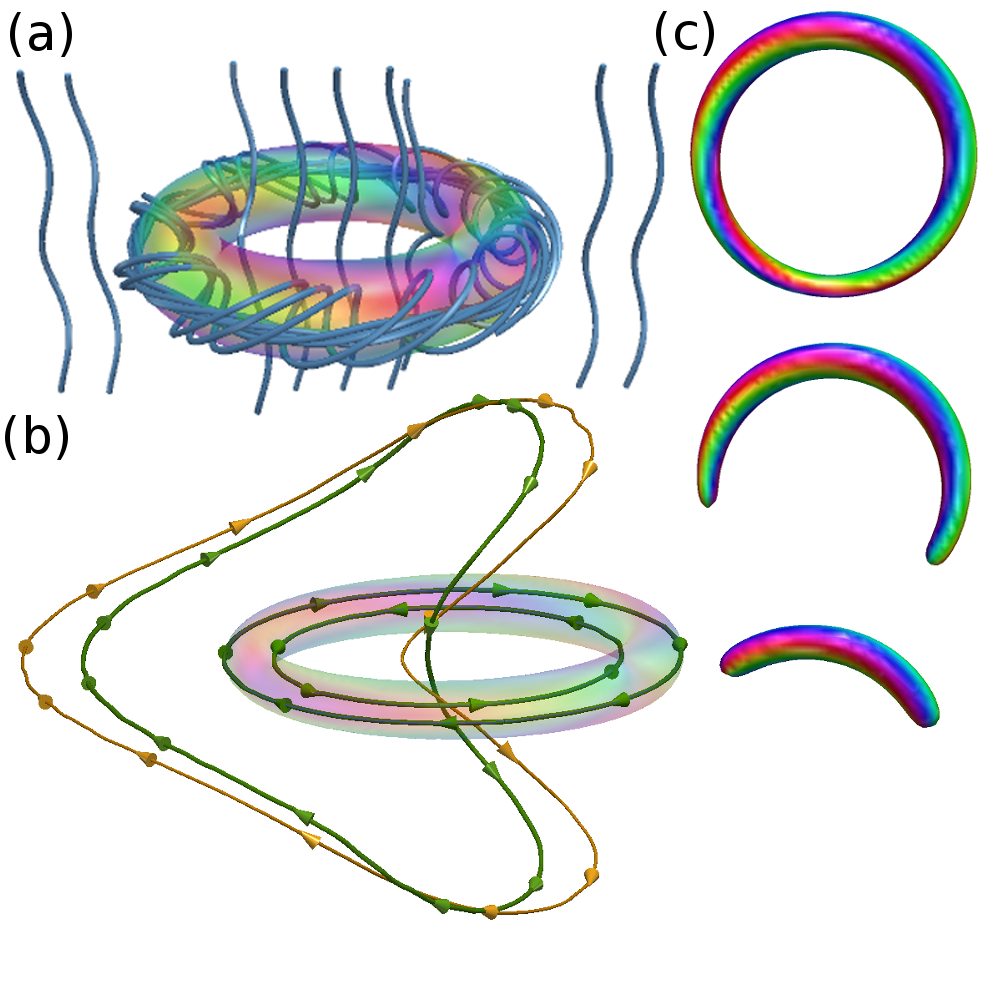
\includegraphics[width=0.7\textwidth]{\TwistBendFigures/hopf.png}
    \caption{}.
    \label{fig:Hopf}
\end{figure}
